\documentclass[10pt]{IEEEtran}
\usepackage{amsmath}
\usepackage{graphicx}
\usepackage{xfrac}
\newcommand{\Pk}{$\textrm{P}_k$}
\title{Aircraft Trajectory Prediction using Recurrent Neural Networks}
\author{\IEEEauthorblockN{Capt Justin Merrick}\\
\IEEEauthorblockA{\textit{Dept. of Aeronautics and Astronautics}\\
\textit{Air Force Institute of Technology}\\
WPAFB, OH\\
justin.merrick@afit.edu
}}

\begin{document}
\maketitle
\section{Introduction}
Aircraft trajectory prediction is of great importance to a number of Air Force doctrine areas such as Offensive and Defensive Counter-air. While the equations of motion for an aircraft are well understood and these can be applied to predict aircraft trajectory, such as in a simulator, not all of the factors present in these equations are observable to a third party. Currently, radars often use some trajectory prediction in order to determine whether a particular return is a new object or an object that has already been tracked. While these prediction algorithms are very effective for their purpose of distinguishing between tracks, they can be fooled, so there is room for a lightweight and fast trajectory prediction algorithm that could be used in applications where size, weight, computing power, and time constraints prevent a more robust prediction from being used.

Due to the non-linear nature of the equations of motion, it is hypothesized that in a partially observable environment (i.e. where not all parameters of the equations of motions are known), an artificial neural network may be able to predict the future location of a target. This paper investigates several neural network architectures, primarily using recurrent layers, in an effort to outperform a baseline trajectory prediction function based on linear regression.

\section{Background}
\subsection{Aircraft Equations of Motion}
The equations of motion for aircraft can be expressed as two sets of three equations. The first three, shown in Equation \ref{eq:lon_eom}, are known as the longitudinal equations of motion and represent movement in the body-fixed $xz$ plane and rotation about the body-fixed $y$ axis. The second set, shown in Equation \ref{eq:lat_eom}, are known as the lateral-directional equations of motion and consist of movement along the body-fixed $y$ axis and rotation about the body-fixed $x$ and $z$ axes. These are further augmented by the kinematic equations relating the body axis rates to the Euler rates, as shown in Equation \ref{eq:kinematics} \cite{Yechout}. These are shown to illustrate the scope of the problem in determining the trajectory of an aircraft and to demonstrate that, if the environment is even slightly partially observable, the effects cascade through most of the equations. Fortunately, in the use case discussed in this paper, that of aircraft trajectory tracking where we are additionally constrained by time, the accuracy must be only good enough to distinguish between potential tracks.

\begin{equation}
    \begin{split}
        m\left(\dot{U}+QW-RF\right) &= -mg\sin \Theta \\
        &\quad+ \left(-D\cos \alpha + L\sin\alpha\right)\\
        &\quad+ T \cos\Phi_T \\
        \dot{Q}I_{yy} -PR\left(I_{zz}-I_{xx}\right)&\\
         + \left(P^2-R^2\right)I_{xz} &= M_A + M_T \\
        m\left(\dot{W}+PV-QU\right) &= mg\cos\Phi\cos\Theta \\
        &\quad+ \left(-D\sin\alpha - L\cos\alpha\right)\\ &\quad-T\cos\Phi_T \\
    \end{split}
    \label{eq:lon_eom}
\end{equation}
\begin{equation}
    \begin{split}
        \dot{P}I_{xx} + QR\left(I_{zz}-I_{yy}\right) - \left(\dot{R} + PQ \right)I_{xz} &= L_A + L_t \\
        m\left(\dot{V} + RU - PW\right) &= mg\sin\Phi\cos\Theta\\
        &\quad + F_{A_y} + F_{T_y} \\
        \dot{R}I_{zz} + PQ\left(I_{yy}-I_{xx}\right) + \left(QR - \dot{P}\right)I_{xz} &= N_A + N_T \\
    \end{split}
    \label{eq:lat_eom}
\end{equation}

\begin{equation}
    \begin{split}
        P &= -\sin\Theta\dot{\Psi} + \dot{\Phi} \\
        Q &= \sin\Phi\cos\Theta\dot{\Psi} + cos\Phi\dot{\Theta} \\
        R &= \cos\Phi\cos\Theta\dot{\Psi} - \sin\Phi\dot{\Theta} \\
    \end{split}
    \label{eq:kinematics}
\end{equation}

\subsection{Baseline}
For this paper, the partially observable state of the aircraft available to third pary observer such as a radar or camera will be considered to be the position, given by latitude, longitude, and altitude, the velocity of the aircraft in all three axes, represented above in the body-fixed axis by $U$, $V$, and $W$, and the Euler angles (roll, pitch, and yaw), represented by $\Phi$, $\Theta$, and $\Psi$. These same quantities were available to the baseline linear regression solution. The baseline time differenced these quantities and used stepwise regression to identify statistically relevant terms and resulted in a set of 3 models, one for latitude, longitude, and altitude. These models. These structure of these models is shown in Equation \ref{eq:baseline}. Here roll and pitch are represented as above and latitude, longitude, and altitude are abbreviated as $Lat$, $Lon$, and $Alt$. A $Y$ prefix represents the future value being solved (the endogenous variable) for while a single variable following an exogenous variable (e.g. $\Phi1$) represents the value of the variable at a timestep either at the current time step ($t=0$) or in the past ($t=-1$). Two digits (e.g. $Lat01$) represents the difference between the variable at the current time step and its value at the digits timestep in the past. The baseline was able to achieve excellent performance, with mean-squared error on the training and test data as shown in Table \ref{t:baseline_mse} and prediction intervals of about 5 meters or less \cite{baseline}.

\begin{equation}
    \begin{split}
        YLat&\sim 1+\Phi1+Lat01+Lat03+Lon03+Alt03\\
        &\quad+\Phi0:Lat01+\Theta1:Lat01+\Theta0:Lat03\\
        &\quad+\Phi0:Lon01+\Phi1:Lon01+\Phi1:Lon02\\
        &\quad+\Phi0:Alt02+\Theta0:Alt02+\Phi0:Alt03+\Theta0^2\\
        &\quad+Lat01^2+Lon02^2+Lon03^2+Alt01^2\\
        YLon&\sim 1+\Phi1+Lon01+Lon03+\Phi0:Lat01\\
        &\quad+\Phi0:Lat02+\Theta0:Lon01+Lat02:Lon01\\
        &\quad+\Phi0:Lon02+\Theta1:Lon03+Lat01:Lon03\\
        YAlt&\sim 1+\Phi0+\Phi1+\Theta0+\Theta1+Alt01+Alt02\\
        &\quad+\Theta0:\Theta1+\Theta0:Lon01+\Phi0:Alt01\\
        &\quad+\Theta0:Alt03+\Theta1:Alt03+\Theta1^2+Lon03^2\\
        &\quad+Alt01^2+Alt02^2
    \end{split}
    \label{eq:baseline}
\end{equation}

\begin{table}
    \caption{Baseline $MSE$ and $MSPR$}
    \centering
    \begin{tabular}{ccc}
        \hline
        &\textbf{Model-building $MSE$}&$MSPR$\\
        \hline
        Latitude&1.071&1.330\\
        Longitude&1.754&1.585\\
        Altitude&0.596&0.473\\
        \hline
    \end{tabular}
    \label{t:baseline_mse}
\end{table}

\section{Methodology}
\subsection{Data}
The data used in training the proposed neural network is the same that was used for the baseline. It consists of four flights of a fixed-wing small unmanned aircraft system (sUAS). The flights were conducted in the same week and consisted of basic checkout maneuvers at a variety of altitudes, speeds, and headings. These maneuvers were then captured in a telemetry log by the ground control station. The logs for each flight contain a multitude of parameters about the flight, a small fraction of which were used as the input data, as discussed above. Initially, these variables came in a multitude of non-intuitive units, so they were standardized to SI units. The input variables to both the baseline model and neural network, along with their standardized units were:

\begin{itemize}
    \item $vx$ - rate of change of longitude(m/s)
    \item $vy$ - rate of change of latitude(m/s)
    \item $vz$ - rate of change of altitude(m/s)
    \item $\phi$  - roll (rad)
    \item $\theta$  - pitch (rad)
    \item $\psi$ (rad)
    \item $Lat$- latitude (deg)
    \item $Lon$ - longitude (deg)
    \item $Alt$ - altitude (m)
\end{itemize}

These data were then used to predict $Lat$, $Lon$, and $Alt$ at future timesteps. The baseline predicted 1 second in the future, the neural network model initially mimicked this choice for comparative purposes. 

The baseline used two measures of success, which were mimicked in the analysis of the neural network. Mean-squared error ($MSE$) was used as a measure of the error in the predictions. To mimic the three separate models of the baseline, $MSE$ was calculated for each quantity as well as the whole neural network. A 95\% confidence interval was also calculated on the test data in order to give spatial meaning to the accuracy expressed by $MSE$.

Of the four flights available, the baseline used only three, using one as a training set, a second as validation, and a third as a test set. Due to the need for additional training data for a neural network when compared to a linear regression, the fourth flight was added to the training set. To maximize the use of the training data, a generator was created that could take subsets of a random choice between the training flights.

In addition to standardizing the units, the data underwent three main preprocessing steps. First, the data from before takeoff and after landing were trimmed from each flight. Takeoff and landing were determined by the first and last time the absolute value of the z-velocity, $vz$, grew greater than $0.5 \sfrac{m}{s}$. Points outside of the range were discarded. Second, the data was normalized. Rather than choosing a baseline for each value and then forcing zero mean and unit standard deviation, normalizing factors were chosen via the performance of the aircraft in question and the nature of the data. This should allow for relatively easy adaptation to other aircraft. The normalization factors used were:

\begin{itemize}
    \item $vx_{norm} = \sfrac{vx}{50} $
    \item $vy_{norm} = \sfrac{vy}{50} $
    \item $vz_{norm} = \sfrac{vz}{50} $
    \item $\phi_{norm} = \sin\phi , \cos\phi$
    \item $\theta_{norm} = \sin\theta, \cos\theta$
    \item $\psi_{norm} = \sin\psi, \cos\psi$
    \item $Lat_{norm} = \sfrac{110.574\left(Lat-Lat_{initial}\right)}{0.3}$
    \item $Lon_{norm} = \sfrac{111.320\cos Lat_{initial}\left(Lon-Lon_{initial}\right)}{0.3}$
    \item $Alt_{norm} = \sfrac{Alt-Alt_{initial}}{1000 * 130}$
\end{itemize}

The assumptions made on aircraft performance by these factors were:

\begin{itemize}
    \item Aircraft max speed $\approx 50 \sfrac{m}{s}$
    \item Maximum distance from start point $0.3 km$
    \item Maximum altitude $130 m$
\end{itemize}

The first was chosen by considering the type of target and then by examining the data after the value was chosen to ensure that it was an accurate assumption. The second was chosen by examining the airspace that the aircraft was flown in, and the third was chosen due to airspace regulations (commercial sUAS flight in the national airspace limited to $400 ft \left(\approx 122m\right)$ AGL, plus a buffer. It is important to note that because these factors were chosen without explicit knowledge of the data, different normalization factors could be chosen for a different trajectory prediction task. The normalization factor of $\sin$ and $\cos$ was chosen for the angles to prevent a discontinuity at $-\pi$ and $\pi$, the limits of the values. Using $\sin$ and $\cos$ smooths this discontinuity.

Third, GPS dropouts were addressed. During initial examination of the data, it was noted that there were several occasions in which the values for $Lat$, $Lon$, and $Alt$ would go to zero for several seconds before resuming. This was determined to be due to loss of GPS track. In order to account for these wild shifts in value, which resulted in data far outside the desired normalized band, a value hold was put into place, wherein the last value before the dropout was maintained until a new value in the normalized range was seen. While this still results in some inaccurate data, the value changes are now more manageable and the inaccuracies are minimized.

\subsection{Models}
As shown in Table \ref{t:baseline_mse}, the baseline $MSE$ ranges between $0.596$ and $1.754$. This was the initial goal to beat. Therefore, the loss function selected for all of the models tested was $MSE$, with additional metrics being reported to calculate the $MSE$ of latitude, longitude, and altitude. Due to the timeseries nature of the data, it was initially hypothesized that a recurrent neural network (RNN) would be appropriate to generate trajectory predictions. This RNN was then paired with a time-distributed dense layer to yield predictions of latitude, longitude, and altitude at one second in the future. A time distributed topology was chosen in order to allow for predictions to be made from a single sample. This is in contrast to the baselines, which requires 4 samples, including the current one, to generate a prediction. The downside to this topology being that there is a warm-up period during which the predictions may not be as accurate.

A topology which was not time-distributed was examined, but the results were found to be less accurate than the time-distributed model. The time-distributed model was expanded from an initial RNN and Dense layer to the topology shown in Figure \ref{f:topology} which includes a dense layer before and after a series of LSTM layers as feature extraction layers. Other topologies considered, but ultimately discarded were a pure RNN model, with only a single dense output layer, a model with 1D convolution feature extraction, and a multi-head model that generated separate outputs for $Lat$, $Lon$, and $Alt$, to mimic the three models of the baseline. As can be seen in Figure \ref{f:topology}, the Keras \textit{CuDNNLSTM} was chosen. This is an LSTM layer tha is optimized for running on a GPU, allowing for quicker training times. This comes at the cost of dropout and recurrent dropout being natively available in the layers. Fortunately, these features were not ultimately needed. A \textit{ReLu} activation was selected for each of the dense layers, $\tanh$ for each of the LSTM layers, and the final model used layers of the sizes shown in Table \ref{t:layer_sizes}. \textit{RMSProp} was chosen as the optimizer.

\begin{figure}
    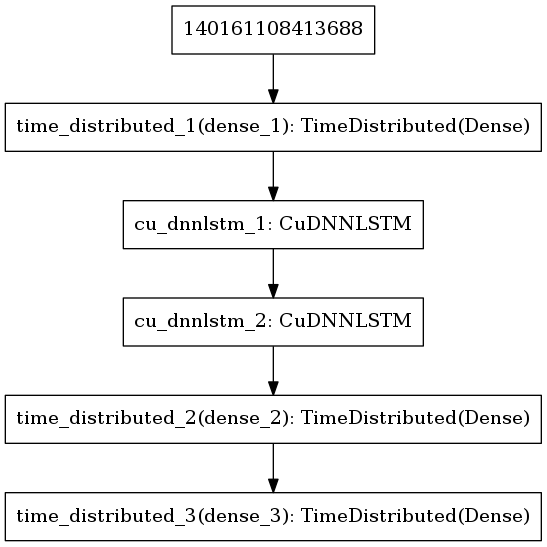
\includegraphics[width=0.95\columnwidth]{model_topology.png}
    \caption{Topology of final model}
    \label{f:topology}
\end{figure}

\begin{table}
    \caption{Layer sizes in final model}
    \centering
    \begin{tabular}{cc}
        \hline
        \textbf{Layer Type} & \textbf{Layer Size} \\
        \hline
        Dense & 64\\
        LSTM & 64\\
        LSTM & 64\\
        Dense & 32\\
        Dense & 3\\
        \hline
    \end{tabular}
    \label{t:layer_sizes}
\end{table}

Following the determination of this architecture, the hyperparameters were tuned. Particularly, the batch size, the number of batches per epoch, and the number of epochs trained. Learning rate was initialized at 0.001 and a callback was used to reduce the learning rate by a factor of 10 after not improving for six epochs. This callback helped to prevent overfitting and helped to decrease the loss further. Additionally, each time a new best model, based on validation loss, was created, it was saved. During hyperparameter tuning, the batch size, which in this case equated to the number of timesteps, and the number of batches per epoch were varied to keep their product around 6000, this prevented too much reuse of the training data. The final hyperparameters are shown in Table \ref{t:hyperparams}.

\begin{table}
    \caption{Final hyperparameters}
    \centering
    \begin{tabular}{cc}
        \hline
        \textbf{Hyperparameter} & \textbf{Value}\\
        \hline
        Batch size (timesteps) & 100\\
        Batches per epoch & 60\\
        Epochs & 100\\
        Initial learning rate & 0.001\\
        \hline
    \end{tabular}
    \label{t:hyperparams}
\end{table}

Once the hyperparameters were tuned, an additional setting was varied to determine the model's predictive capability. The number of timesteps ahead that the target values were sampled was varied between 1 and 5 seconds. Following the training phase, the model was evaluated on the entire validation flight in sequential order. Finally, the model was evaluated on the test flight in the same manner and was also used to generate predicitions for error comparison. 

\section{Results}
The results from the model training process are shown as a training dataset loss history and a validation dataset loss history in Figure \ref{f:loss}. There appears to be significant noise in the training loss, but it should be noted that these oscillations are on the order of 0.04. The full flight validation and test $MSE$ are shown in Table \ref{t:flight_mse}. 

A major limitation of the baseline was its ability to only predict 1 second into the future. the trained model was evaluated against its ability to predict up to 5 seconds in the future and the results were compared to a model trained with the targets farther into the future, these results are summarized in Table \ref{t:time_study}.

\begin{figure}
    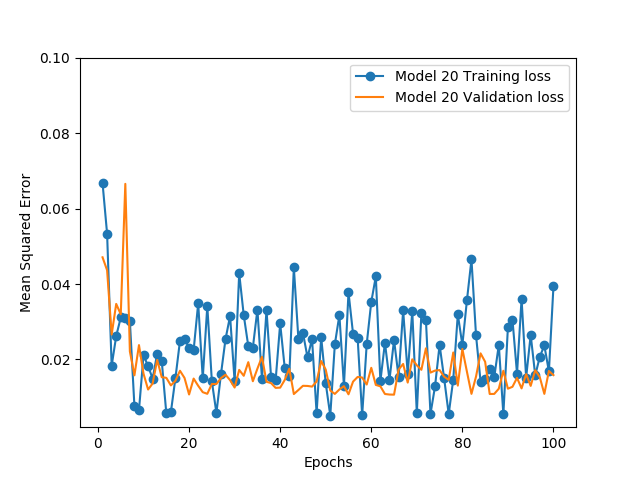
\includegraphics[width=0.95\columnwidth]{training_hist.png}
    \caption{Batch-generated Training and Validation Loss}
    \label{f:loss}
\end{figure}

\begin{table}
    \caption{$MSE$ for Full-flight Validation and Test Data}
    \centering
    \begin{tabular}{ccc}
        \hline
        \textbf{Metric}&\textbf{Validation}&\textbf{Test}\\
        \hline
        $MSE$ & 0.0161& 0.0212\\
        $Lat$ $MSE$ & 0.0482& 0.0507\\
        $Lon$ $MSE$ & 0.0403& 0.0431\\
        $Alt$ $MSE$ & 0.0283& 0.0312\\
        \hline
    \end{tabular}
    \label{t:flight_mse}
\end{table}

\begin{table}
    \caption{Prediction capabilities out to t+5 seconds}
    \centering
    \begin{tabular}{ccc}
        \hline
        \textbf{Prediction time}& \textbf{t+1 Model $MSE$} & \textbf{t+x $MSE$}\\
        \hline
        t+1 & 0.0212 & 0.0212\\
        t+2 & 0.0120 & 0.0106\\
        t+3 & 0.0152 & 0.0209\\
        t+4 & 0.0221 & 0.0359\\
        t+5 & 0.0323 & 0.0421\\
        \hline
    \end{tabular}
    \label{t:time_study}
\end{table}

The previous tables and figure dealt with normalized errors. In Figure \ref{f:errors}, the model was used to predict values based off of the test data, the errors compared on a per timestep basis, and then converted back into the original units before graphing. Additionally, 95\% confidence intervals were calculated on the errors in original units. These are shown in Table \ref{t:conf_int}. For comparison, Figure \ref{f:baseline} shows the error and confidence intervals on the test set from the baseline.

\begin{figure}
    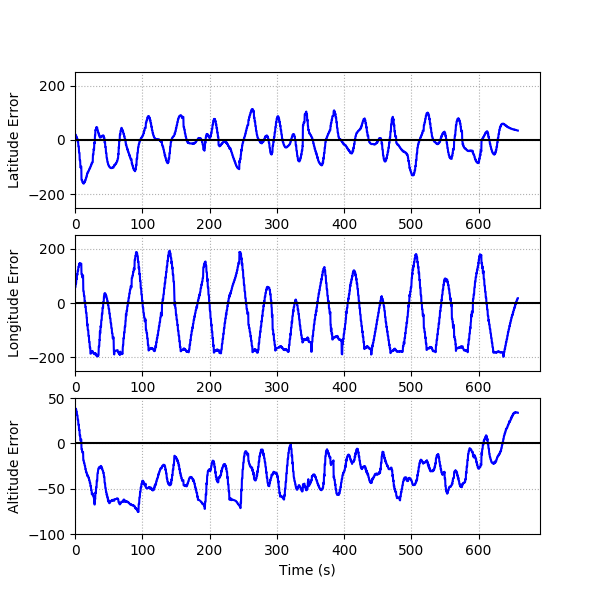
\includegraphics[width=0.95\columnwidth]{test_error.png}
    \caption{Prediction Error on Test Data}
    \label{f:errors}
\end{figure}

\begin{table}
    \caption{95\% confidence intervals on Test Data}
    \centering
    \begin{tabular}{ccc}
        \hline
        &\textbf{Lower}&\textbf{Upper}\\
        $Lat$ (m)& -112.9 & 99.1\\
        $Lon$ (m)& -270.6 & 160.3\\
        $Alt$ (m)& -76.0 & 8.65\\
        \hline
    \end{tabular}
    \label{t:conf_int}
\end{table}

\begin{figure}
    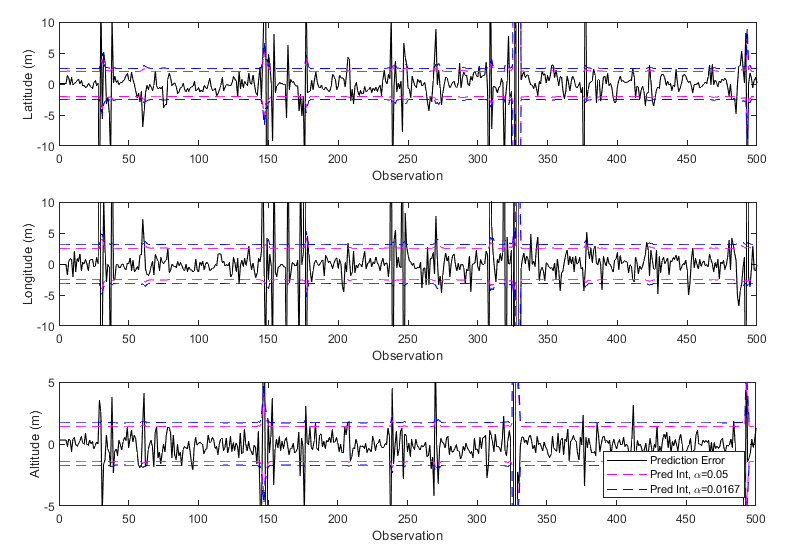
\includegraphics[width=0.95\columnwidth]{untrim_predict.png}
    \caption{Baseline performance on test data with GPS dropouts}
    \label{f:baseline}
\end{figure}

\section{Discussion}
 The successful training of the model in Figure \ref{f:loss}, though noisy, still demonstrates an $MSE$ value of $<0.01$ in normalized units. This value represents the lowest obtained from training with multiple topologies and hyperparameters. This accuracy held when trainsitioning from the batch driven training environment to a full flight evaluation, but was degraded by 24\% when evaluated against the test data.

The model also showed that it could perform similarly at predictions out to t+3 seconds, before degrading by about 25\% in $MSE$ when evaluated against t+4 seconds data. In all cases except for t+2 seconds, the model was able to outperform a model trained with the data at that time offset, though the differences were small.

While these values at first glance indicate a useful model, the large normalization factors applied during preprocessing cause false confidence in the performance. In order to convert back to the original units of meters, the predicted $Lat$ and $Lon$ must be multipled by 300 and the $Alt$ by 130. This leads to $O\left(4\right)$ increases in the $MSE$, indicating that the predictive capability of the model is poor. This is supported by Figure \ref{f:errors} and Table \ref{t:conf_int}. All of the errors calculated on the test set show a periodic nature of around $0.03 Hz$. $Lat$ and $Lon$ seem to have no bias, while $Alt$ displays a bias to underestimate the next altitude. $Lon$ has the largest magntide or errors, $Alt$ the smallest. The negative bias of the $Alt$ errors puts a number of predicted observations very close to the ground, potentially leading to not just only poor predictions, but impossible ones without a crash. The periodic nature of the errors may indicate that the $\sin$ and $\cos$ normalization of the Euler angles destroyed some of the interaction data between the different angles.

It may also have been that the time distributed model is an insufficient topology to capture the nonlinearities present in the equations of motion and a different architecture needed to be explored further. Regardless of the source of the inaccuracies, the neural network model developed was unable to improve upon the baseline model using a linear regression approach.

\section{Conclusion}
To solve the problem of trajectory prediction by using observable variables, a neural network model was proposed utilizing a time distributed approach with fully-connected feature extraction layers and LSTM layers to create a state history. The time distributed approach allowed predictions to be created from a single observation. Multiple architectures were investiaged prior to the selection of this one and, following selections, hyperparameter tuning was conducted to maximize the performance of the model. Despite this tuning, the performance obtained was poor, with confidence interval widths of greater than 80 meters. In comparison, the baseline utilizing linear regression was able to achieve less than 10 m confidence interval widths.

While this particular architecture was unable to meet the baseline, future work to improve upon the solution could include the investigation of additional architectures, the investigation of the cause of the periodic errors identified during evaluation, and the expansion of the dataset to include aircraft of multiple performance envelopes to check the veracity of the hypothesis that the normalized model may have more generalizable capabilities.

\bibliographystyle{IEEEtran}
\bibliography{IEEEabrv,ReportBib}

\end{document}
